% =============================================================================
% Chapter 2 — System Architecture
% =============================================================================
\chapter{Technical Description}

\section{Global Architecture}

SecurAccess adopts a modular \textbf{MVC} (Model--View--Controller) architecture, structured into distinct layers:

\begin{infobox}[Layered Architecture]
\begin{itemize}[nosep]
    \item \textbf{Presentation Layer (UI)} — PyQt5 Pages: Login, Welcome, Admin Dashboard, Access Denied, Unknown Face, Enrollment
    \item \textbf{Controller Layer} — \texttt{AuthController} orchestrates the authentication pipeline
    \item \textbf{Service Layer} — Business logic: Auth, Camera, FaceDetection, FaceBiometric, Log, Watermark, Alert, Email, Enrollment, Upgrade
    \item \textbf{Data Layer} — SQLite via \texttt{DatabaseService}, \texttt{dataclass} models
\end{itemize}
\end{infobox}

\subsection{Architecture Diagram}

\begin{figure}[H]
\centering
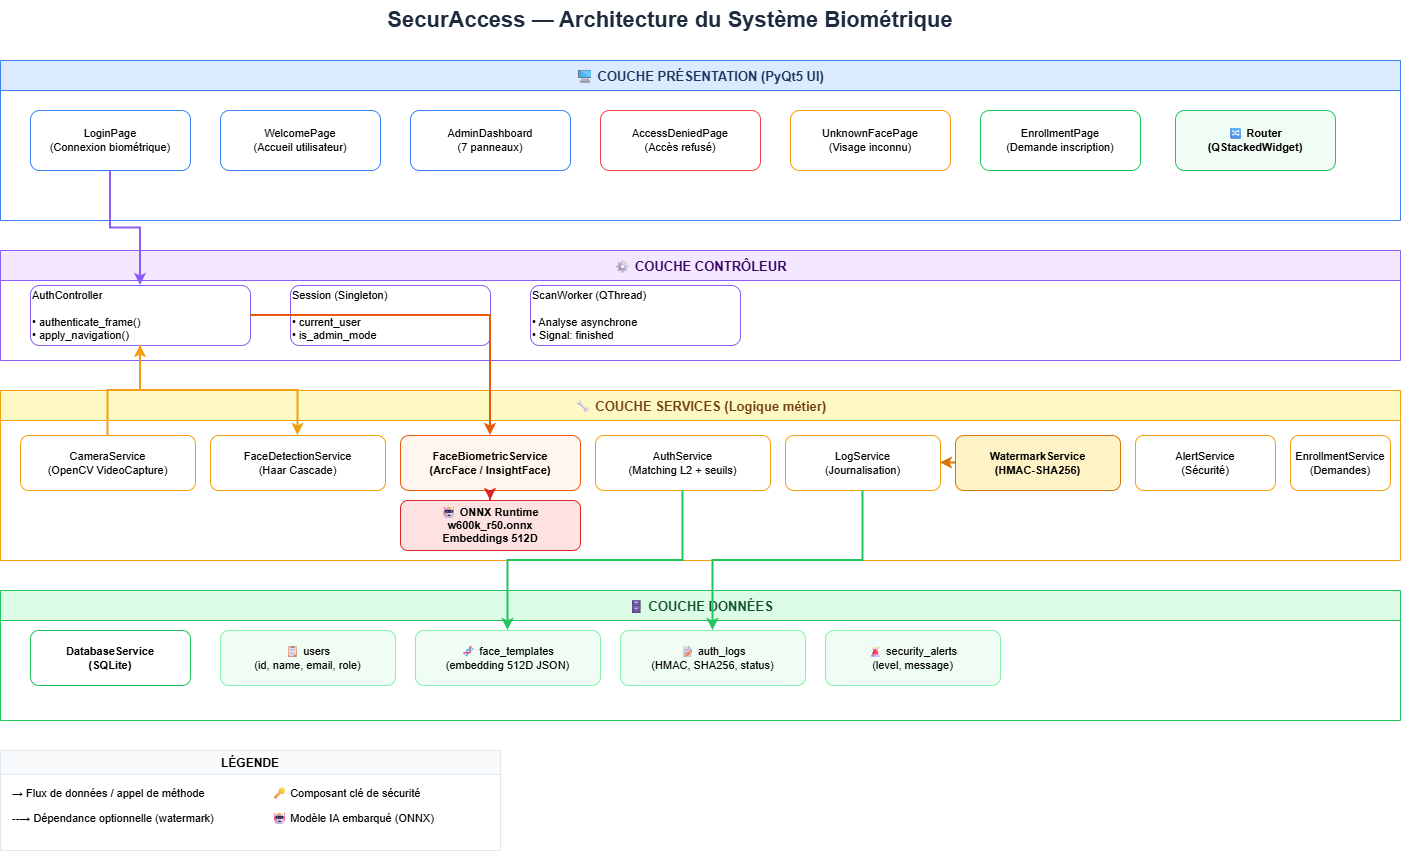
\includegraphics[width=0.95\textwidth]{images/architecture_securaccess.png}
\caption{Global architecture diagram of the SecurAccess system}
\label{fig:archi-globale}
\end{figure}

\subsection{Project Structure}

\begin{lstlisting}[language={}, caption={Project Tree}]
SecurAccess/
|-- main.py                    # Entry point
|-- data/
|   |-- securaccess.db         # SQLite Database
|   |-- faces/                 # Enrolled face images
|-- app/
|   |-- core/
|   |   |-- router.py          # Navigation (QStackedWidget)
|   |   |-- session.py         # User session (Singleton)
|   |-- controllers/
|   |   |-- auth_controller.py # Authentication pipeline
|   |-- models/
|   |   |-- user.py            # User model + roles
|   |   |-- auth_result.py     # Authentication result
|   |   |-- face_detection_result.py
|   |   |-- enrollment_request.py
|   |-- services/
|   |   |-- auth_service.py         # Facial authentication
|   |   |-- face_detection_service.py  # Haar Cascade detection
|   |   |-- face_biometric_service.py  # ArcFace embeddings
|   |   |-- camera_service.py       # Webcam management
|   |   |-- database_service.py     # SQLite access
|   |   |-- watermark_service.py    # HMAC-SHA256 watermarking
|   |   |-- log_service.py          # Watermarked logging
|   |   |-- alert_service.py        # Security alerts
|   |   |-- email_alert_service.py  # Email notifications
|   |   |-- enrollment_service.py   # Enrollment requests
|   |   |-- upgrade_service.py      # Upgrade requests
|   |-- ui/
|   |   |-- login_page.py           # Login page
|   |   |-- welcome_page.py         # User home page
|   |   |-- access_denied_page.py   # Access denied
|   |   |-- unknown_face_page.py    # Unknown face
|   |   |-- enrollment_page.py      # Enrollment form
|   |   |-- admin/                   # Admin dashboard (7 panels)
|   |   |-- components/              # Reusable components
|   |   |-- dialogs/                 # Modal dialogs
|   |-- resources/
|       |-- styles.py           # Theme and color palette
|-- scripts/
    |-- enroll_admin.py         # Webcam enrollment script
\end{lstlisting}

\section{Database Schema}

The system uses \textbf{SQLite} with four main tables:

\begin{table}[H]
    \centering
    \begin{tabularx}{\textwidth}{llX}
        \toprule
        \textbf{Table} & \textbf{Primary Key} & \textbf{Description} \\
        \midrule
        \texttt{users}            & \texttt{id} (AUTO)  & Registered users (face\_id, name, email, role, status) \\
        \texttt{face\_templates}  & \texttt{id} (AUTO)  & 512D ArcFace embeddings stored in JSON, linked to \texttt{users.id} \\
        \texttt{auth\_logs}       & \texttt{id} (AUTO)  & Authentication logs with HMAC watermark and SHA256 hash \\
        \texttt{security\_alerts} & \texttt{id} (AUTO)  & Security alerts by level (critical, warning, info) \\
        \bottomrule
    \end{tabularx}
    \caption{SQLite database tables}
\end{table}

\screenshotplaceholder[1]{Database relational schema}{schema-bdd}

\section{Navigation System}

Navigation is managed by a \textbf{Router} (Singleton pattern) which controls a \texttt{QStackedWidget}. All pages are instantiated once at startup and stacked. Navigation is done by name:

\begin{lstlisting}[language=Python, caption={Navigation example}]
Router.get_instance().navigate("welcome")  # Displays the welcome page
Router.get_instance().go_back()            # Go back
\end{lstlisting}

Registered pages: \texttt{login}, \texttt{welcome}, \texttt{access\_denied}, \texttt{unknown\_face}, \texttt{enrollment}, \texttt{admin\_dashboard}.

\section{Session Management}

The user session is a \textbf{Singleton} (\texttt{Session}) that stores the logged-in user and their mode (admin or standard user). It is accessed by all pages to adapt the display and permissions.

\section{Hierarchical Role System}

The system implements five role levels with a numerical hierarchy:

\begin{table}[H]
    \centering
    \begin{tabular}{lcc}
        \toprule
        \textbf{Role} & \textbf{Level} & \textbf{Access} \\
        \midrule
        Admin        & 100 & Full access + Administration dashboard \\
        Ultimate     & 50  & All user sections \\
        Pro          & 30  & Pro + User sections \\
        User         & 10  & Basic sections only \\
        Unauthorized & 0   & Recognized but access revoked \\
        \bottomrule
    \end{tabular}
    \caption{Role hierarchy in SecurAccess}
\end{table}
